% "{'classe':('PSI'),'chapitre':'slci_correcteurs','type':('colle'),'titre':'Réglage d\\'un correcteur P et d\\'un correcteur à avance de phase', 'source':'Équipe PT - La Martinière Monplaisir','comp':('C1-02','C2-04'),'corrige':False}"
%\setchapterimage{bandeau}
\chapter*{Colle \arabic{cptColle} \\ 
Réglage d'un correcteur P et d'un correcteur à avance de phase -- 
\ifprof Corrigé \else Sujet \fi}
\addcontentsline{toc}{section}{Colle \arabic{cptColle} :
Réglage d'un correcteur P et d'un correcteur à avance de phase -- 
\ifprof Corrigé \else Sujet \fi}

\iflivret \stepcounter{cptColle} \else
\ifprof  \stepcounter{cptColle} \else \fi
\fi

\setcounter{question}{0}
\marginnote{Équipe PT -- La Martinière Monplaisir.}
\marginnote[1cm]{
\UPSTIcompetence[2]{C1-02}
\UPSTIcompetence[2]{C2-04}}


%\begin{marginfigure} [4cm]
%\includegraphics[width=\linewidth]{fig_01a}
%\end{marginfigure}



On considère un système de fonction de transfert est :  $G(p)=\dfrac{K}{(p+1)^3}$ placé dans une boucle de régulation à retour unitaire. On souhaite une marge de phase supérieure à 45\degres.

\question{Tracer le schéma-blocs associé au système.}

\question{Exprimer l'écart de statique et l'écart de trainage.}


\question{Définir la condition de stabilité théorique du système.}


On note $t_m$ le temps de montée du système en BF avec  $t_m\simeq \dfrac{3}{\omega_{\text{co}}}$ et $\omega_{\text{co}}$ est la pulsation de coupure à \SI{0}{dB} du système en BO.  


\question{Calculer la valeur $K$ qui assure, en boucle fermée, un temps de montée de \SI{2,15}{s}.}

\question{Calculer pour cette valeur de $K$ la marge de phase.}

\question{En déduire l'expression de la fonction de transfert du correcteur à avance de phase $C(p)=K_a\dfrac{1+aTp}{1+Tp}$ qu'il faut introduire dans la chaîne directe.  }


\ifprof

\begin{center}
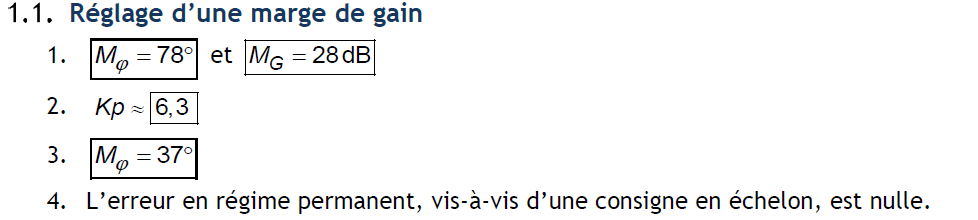
\includegraphics[width=\linewidth]{cor_01}
\end{center}
\else
\fi
